\documentclass[10pt,a4paper]{article}
\usepackage[margin=21mm,headheight=13pt]{geometry}
\usepackage[T1]{fontenc}
\usepackage[utf8]{inputenc}
\usepackage{lmodern,microtype}
\usepackage{amsmath,amssymb,amsthm,mathtools}
\usepackage{graphicx,booktabs,tabularx,array,enumitem}
\usepackage[dvipsnames]{xcolor}
\usepackage{hyperref,fancyhdr}
\hypersetup{colorlinks=true,linkcolor=MidnightBlue,citecolor=MidnightBlue,urlcolor=MidnightBlue,
 pdftitle={Prepared recovery as a certificate for rare failure},pdfauthor={Astra research construction}}
\urlstyle{same}
\setlength{\parskip}{4pt}
\setlength{\parindent}{0pt}
\setlist{topsep=3pt,itemsep=2pt,parsep=1pt,leftmargin=*}
\setlength{\emergencystretch}{2em}
\pagestyle{fancy}\fancyhf{}
\fancyhead[L]{\small Prepared recovery and rare failure}
\fancyhead[R]{\small 5 November 2026}
\fancyfoot[C]{\thepage}
\newtheorem{theorem}{Theorem}[section]
\newtheorem{lemma}[theorem]{Lemma}
\newtheorem{proposition}[theorem]{Proposition}
\newtheorem{corollary}[theorem]{Corollary}
\theoremstyle{definition}\newtheorem{assumption}[theorem]{Assumption}
\newtheorem{remark}[theorem]{Remark}
\newcommand{\E}{\mathbb E}
\newcommand{\Prob}{\mathbb P}
\newcommand{\Var}{\operatorname{Var}}
\newcommand{\diag}{\operatorname{diag}}
\newcommand{\TV}{\operatorname{TV}}
\newcommand{\cE}{\mathcal E}
\newcommand{\one}{\mathbf 1}
\newcommand{\eps}{\varepsilon}
\newcommand{\ip}[2]{\langle #1,#2\rangle_\pi}
\newcommand{\revhash}{5cfc803599d9f95cfa0a55896fb580e77567e162}
\begin{document}
\begin{center}
{\LARGE\bfseries Prepared recovery as a certificate for rare failure}\\[5pt]
{\large Unknown local mechanisms in reversible thermal registers}\\[7pt]
{Astra research construction \quad $\cdot$ \quad 5 November 2026}
\end{center}

\begin{abstract}
An unobserved failure mechanism can invalidate a long-lifetime prediction while remaining invisible during short passive observation. We construct an intervention interface for a restricted engineered family in which this ambiguity can be bounded. A register has additive occupation energies, fresh reciprocal local collision ports, and a retained independent refresh backbone. Prepared local inputs expose downhill responses; detailed balance relates them to rare uphill events. The transition support within each declared port is unknown, and rates may vanish. Simultaneous \emph{absolute} response intervals induce a reversible error generator. A local variance bound and product tensorization compare its full Dirichlet form to the native backbone, without enumerating global configurations. We prove a fixed-start mean-first-failure perturbation bound and extend the supplied independent-network computation to correlated dynamics with product equilibrium. The algorithm invokes Karger's all-terminal counting method, includes a constructed failure-conditioned sampler, and covers rare and nonrare branches. Its costs depend on local port size, refresh contrast, initial stationary mass, accuracy, and input bit length; these restrictions remain explicit. A finite-clock collision realization makes the physical endpoint mean exact, and a separate forest bound treats finite ancillary preparation errors under strong, stated QND verification assumptions. Synthetic two-bit and six-bit experiments show consequential cooperative failure routes with no observed uphill cooperative transition. The result is a mathematical construction with numerical evidence, not a hardware demonstration, universal reliability certificate, priority claim, or established civilisation-changing capability.
\end{abstract}

\section{Question, consequence, and scope}

The question is whether an experiment can expose all consequential mechanisms \emph{within a physically specified reach}, sufficiently to infer a rare first-failure mean without waiting for that failure. The operation developed here is a prepared local recovery experiment. It is useful because a thermally suppressed forward event can have an ordinary reverse response, and because the cumulative effect of all still-unseen local responses can be bounded.

Reverse kinetic inference is established: Trendelkamp-Schroer and No\'e combine equilibrium probabilities with downhill trajectories, and TRAM combines biased equilibrium information with short kinetic data \cite{prx2016,tram}. The additional construction here is an unknown-support confidence theorem, a local physical coverage interface, and a complete first-failure calculation for correlated product-invariant dynamics. It uses the supplied P2 computation as machinery \cite{p2}; it does not repeat a validation campaign on that source.

The operational target is the \textbf{first failed registered endpoint}. During a finite quantum collision pulse the register need not have a definite classical occupation. No assertion is made that a continuously monitored physical network remains connected between endpoints. An application whose failure is an in-pulse transient needs a different observable and model.

\paragraph{Main guarantee, informally.}
With the exact architectural conditions below, exhaustive local preparations and ordinary response counts give an interval for the all-working mean first disconnection of a known network. Unknown correlated channels and observed-zero channels are included. At fixed maximum port size and usable refresh and initial-mass parameters, acquisition and computation have polynomial cost. No inverse global failure probability is an execution factor in the rare branch. The conditions are earned for the specified collision architecture; they are not inferred for an arbitrary device from silent observations.

\section{Mathematical model and exact collision interface}

\subsection{Product equilibrium with correlated dynamics}

There are $m$ bits $x\in\{0,1\}^m$. A one denotes a failed or excited component. Let
\begin{equation}
 \pi(x)=\prod_{i=1}^m p_i^{x_i}(1-p_i)^{1-x_i},\qquad 0<p_i<1.
 \label{eq:product}
\end{equation}
The mathematical results permit any $p_i$. The physical occupation construction uses $p_i\le1/2$. A known graph assigns one bit to each edge; the working edges have $x_i=0$. Let $B$ be its disconnected configurations and $A=B^c$. More general nonempty failure sets are allowed in the perturbation theorems, but the efficient counting algorithm below is specifically all-terminal disconnection.

Write
\begin{equation}
 Q=Q_0+\sum_{\alpha=1}^r Q_\alpha,\qquad
 Q_0f(x)=\sum_{i=1}^m\gamma_i\{\E_{Z_i\sim\mathrm{Bern}(p_i)}f(x_{-i},Z_i)-f(x)\}.
 \label{eq:model}
\end{equation}
Every $\gamma_i>0$. The native failure and repair rates are $\gamma_i p_i$ and $\gamma_i(1-p_i)$. Each $Q_\alpha$ acts only on a declared block $S_\alpha$, with $k_\alpha=|S_\alpha|\le k$, and is reversible for the local product law. Its rates depend only on that block state. Any necessary context is part of the block. There may be arbitrary transitions among its $s_\alpha=2^{k_\alpha}$ local states, including simultaneous changes and zeros. Let $D$ be the maximum number of blocks containing a coordinate.

For $\ip fg=\sum_x\pi(x)f(x)g(x)$, the Dirichlet form is
\begin{equation}
 \cE_Q(f,f)=\frac12\sum_{x,y}\pi(x)q(x,y)[f(y)-f(x)]^2.
 \label{eq:form}
\end{equation}
The backbone has gap $\gamma_*:=\min_i\gamma_i$. Adding nonnegative reversible forms cannot reduce it. Thus the full gap is at least $\gamma_*$. A known local-rate upper bound supplies $R\ge2\max_x[-q(x,x)]$, so $\mathsf P=I+Q/R$ is lazy and reversible with gap at least $g=\gamma_*/R$. This computational uniformization is distinct from the physical clock introduced below.

The initial state $x_0\in A$ is known, with $\pi(x_0)\ge\kappa>0$. For all-working initialization, $\kappa=\prod_i(1-p_i)$. Dependence on $\kappa^{-1}$ is a real restriction: it need not be polynomial in $m$. Low-temperature examples can have $\kappa$ bounded away from zero while system failure is exponentially rare.

\subsection{Derivation of an observable local kernel}

A port can be isolated, triggered once, and read at its endpoint. It couples $S_\alpha$ to a fresh ancillary copy. For a truly thermal realization, both have additive energy $H=\sum_{i\in S_\alpha}\Delta_i n_i$ and the ancilla has Gibbs probabilities $\tau$. Assume
\begin{equation}
 [U_\alpha,H_S+H_E]=0,\qquad
 |\langle v,b|U_\alpha|u,a\rangle|^2
 =|\langle u,a|U_\alpha|v,b\rangle|^2.
 \label{eq:reciprocity}
\end{equation}
The latter is probability reciprocity, an explicit extra condition. A sufficient realization is one pulse $U=e^{-itV}$ with $V$ real symmetric in the joint occupation basis and commuting with $H_S+H_E$. Then $U^T=U$. A generic sequence of such noncommuting pulses need not have this property. Energy conservation and a thermal ancilla alone do not guarantee detailed balance for every multilevel thermal operation \cite{eto,collisions}.

At the endpoint, dephase the affected register bits in the occupation basis and discard the ancilla. Starting from an occupation input $u$, the measured kernel is
\begin{equation}
 K_\alpha(u,v)=\sum_{a,b}\tau(a)|\langle v,b|U_\alpha|u,a\rangle|^2.
 \label{eq:kernel}
\end{equation}
Every nonzero amplitude conserves energy, hence
$\pi_{S_\alpha}(u)\tau(a)=\pi_{S_\alpha}(v)\tau(b)$.
Multiplying \eqref{eq:kernel} by $\pi_{S_\alpha}(u)$, using reciprocity, and exchanging $(a,b)$ proves
\begin{equation}
 \pi_{S_\alpha}(u)K_\alpha(u,v)
 =\pi_{S_\alpha}(v)K_\alpha(v,u).
 \label{eq:localdb}
\end{equation}
This sums all internal ancillary pathways. None must be individually identified. Fresh ancillas, endpoint dephasing, and the absence of other idle dynamics give a Markov chain on the observed occupations. The wiring gives locality. A full occupation SWAP with a fresh matching bit implements the backbone refresh.

\subsection{Digital ancillary populations without rare-population sampling}

A stricter interface removes uncertain thermodynamic population calibration. Retain probability reciprocity in \eqref{eq:reciprocity} and require the port to conserve each matched number
\begin{equation}
 N_i=n_i^{\rm register}+n_i^{\rm ancilla},\qquad i\in S_\alpha.
 \label{eq:pairnumber}
\end{equation}
Choose rational $p_i=a_i/d_i\in(0,1/2]$ and digitally request independent ancilla occupations with these probabilities. On every allowed transition, conservation of the $N_i$ implies
$\pi(u)\pi(a)=\pi(v)\pi(b)$ directly. Thus \eqref{eq:localdb} follows without inferring tiny Gibbs populations from occupation counts. The symmetry conserves every additive physical energy of matched pairs. Effective dimensionless energies are $h_i=\log[(1-p_i)/p_i]$.

Exact rational sampling uses fair bits to draw a uniform integer in $\{0,\ldots,d_i-1\}$ by rejection and requests one iff the integer is below $a_i$. Expected bit work is below $2\lceil\log_2d_i\rceil$, with $O(\log d_i)$ storage. It is not proportional to $1/p_i$. A physical requested write is a separate operation; finite fidelity is treated in Section~\ref{sec:factory}. This is an engineered thermal-like reservoir, not an assertion about arbitrary natural baths.

\subsection{Finite physical ticks and exact mean conversion}
\label{sec:clock}

Let $T$ include the longest padded port-index sampling, controller, ancillary preparation, pulse, dephasing, reset, and endpoint-service duration of an operating port. This does not reset the operating register. At each tick select one port with prescribed rational weight $w_j$, execute it, and pad to $T$. Include a null identity index as needed. The actual endpoint kernel is
\begin{equation}
 P=\sum_j w_jK_j,\qquad Q=\frac{P-I}{T}.
 \label{eq:physicalclock}
\end{equation}
The $Q$ in this equality is an \emph{analytical generator}. If $N$ is the first failed endpoint and $t(x)=\E_xN$, then
$(I-P_A)t=\one$. Therefore
\begin{equation}
 \boxed{M_{\rm lab}(x)=T\E_xN=(-Q_A)^{-1}\one(x).}
 \label{eq:exactphysicalmean}
\end{equation}
This is exact for the mean; no continuous-time trajectory equivalence or infinitely precise exponential waiting time is asserted. Native refresh coefficients are $\gamma_i=w_i/T$. A serial implementation must satisfy $\sum_i\gamma_i\le1/T$ before allocating other ports. Fixed per-site refresh as $m$ grows requires additional parallel hardware or a faster clock. Actual clock tolerance contributes a direct multiplicative time uncertainty.

\section{Local acquisition with intervals for unseen channels}
\label{sec:acquisition}

For every port $\alpha$ and every local input $u$, prepare $u$, remove preparation control, disable the other ports, provide a fresh ancilla, execute one native collision, dephase, and read the output. Restore before the next trial. One input row supplies counts for every destination. The local map during calibration must be the operating map; uncalibrated stress left on during the pulse is not a substitute.

Let $n_\alpha$ be a fixed number of trials per input. Orient every unordered pair from the endpoint $u$ with smaller known $\pi_{S_\alpha}(u)$ to the larger-weight endpoint $v$; break ties deterministically. Put $\widehat K(u,v)=N_{uv}/n_\alpha$ and infer the reverse by \eqref{eq:localdb}. For rate scale $\nu_\alpha$ (equal to $w_\alpha/T$ in \eqref{eq:physicalclock}), set
\begin{equation}
 \widehat q_\alpha(u,v)=\nu_\alpha\widehat K(u,v),\qquad
 \widehat q_\alpha(v,u)=\widehat q_\alpha(u,v)
      \frac{\pi_{S_\alpha}(u)}{\pi_{S_\alpha}(v)}.
 \label{eq:fit}
\end{equation}
All fitted off-diagonal rates are nonnegative. Reconstructing different pairs from different rows can slightly violate an individual port's original stochastic row cap, but still defines a valid reversible generator. Either enforce the local stochastic constraints or enlarge the fitted computational uniformization bound accordingly.

Let $J=\sum_\alpha\binom{s_\alpha}{2}$ and choose $L=\log(3J/\alpha_{\rm acq})$. For one oriented probability $z$, Hoeffding gives an interval about $\widehat z$ with half-width
\begin{equation}
 h_\alpha=\sqrt{\frac{L}{2n_\alpha}}.
 \label{eq:hoeffding}
\end{equation}
When $N_{uv}=0$, intersect its upper endpoint with $L/n_\alpha$. The two-sided Hoeffding failure is at most $2e^{-L}$. The additional zero-count failure is at most $e^{-L}$ because $\Prob_z(N=0)\le e^{-n_\alpha z}$. A union bound gives simultaneous coverage at least $1-\alpha_{\rm acq}$. Dependence among multinomial destinations does not invalidate this argument.

\textbf{A zero count is not a zero-rate certificate.} Retain the positive upper interval. Input/output contamination bounded in total variation by $\beta_\alpha$ adds $\beta_\alpha$ to each probability radius. Attempt-weight uncertainty contributes to rate intervals. If finite factories perturb ideal probabilities by at most $\zeta$, include that bias in these acquisition bands before fitting an ideal reversible model; the subsequent operating-factory comparison is separate. These errors cannot be replaced by a sampling confidence statement.

The complete local shot bill is $\sum_\alpha s_\alpha n_\alpha$. To use common probability accuracy $h$, it is
\begin{equation}
 N_{\rm acq}=O\!\left(r2^k h^{-2}\log\frac{r4^k}{\alpha_{\rm acq}}\right).
 \label{eq:acqcount}
\end{equation}
Counts here are fixed in advance. Adaptive stopping requires confidence sequences or a confidence allocation over predetermined stages. No inverse uphill probability occurs in \eqref{eq:acqcount}; local preparation, service, and verification costs must still be paid.

\section{An unknown-support certificate by local tensorization}
\label{sec:tensor}

First hold the product law and backbone exact. For each oriented pair let $d_{\alpha,uv}$ be a valid absolute error radius on $q_\alpha(u,v)$. Define a reversible nonnegative error generator $H_\alpha$ by that rate in the measured direction and by $d_{\alpha,uv}\pi(u)/\pi(v)$ in the reverse direction. Its diagonal makes row sums zero. Set
\begin{equation}
 r_\alpha=\max_u\sum_{v\ne u}H_\alpha(u,v),\qquad
 \rho=\max_i\frac{2\sum_{\alpha:i\in S_\alpha}r_\alpha}{\gamma_i}.
 \label{eq:rho}
\end{equation}
The heterogeneous $r_\alpha$ can use the much smaller zero-count intervals. A common rate radius $\delta_\alpha$ gives $r_\alpha\le(2^{k_\alpha}-1)\delta_\alpha$ because the reverse multiplier is at most one.

\begin{theorem}[Local errors control the full form, including missing support]
\label{thm:tensor}
On the simultaneous acquisition event, for every function $f$ on the full register,
\begin{equation}
 |\cE_Q(f,f)-\cE_{\widehat Q}(f,f)|
 \le \rho\,\cE_0(f,f)\le\rho\,\cE_{\widehat Q}(f,f).
 \label{eq:formcontrol}
\end{equation}
In particular, if $\rho<1$ and $L=\diag(\pi_A)(-Q_A)$ is the killed conductance Laplacian, then
\begin{equation}
 (1-\rho)\widehat L\preceq L\preceq(1+\rho)\widehat L.
 \label{eq:killedloewner}
\end{equation}
There is no common-support or positive-minimum-rate condition on the additional ports.
\end{theorem}

\begin{proof}
For each unordered local pair, the absolute conductance difference is at most its conductance in $H_\alpha$. Hence the absolute difference of local forms is bounded by $\cE_{H_\alpha}$. For a function $h$ on that block, subtract its $\pi_{S_\alpha}$ mean. Reversibility and $(a-b)^2\le2a^2+2b^2$ give
\[
 \cE_{H_\alpha}(h,h)
 \le2\sum_u\pi_{S_\alpha}(u)h(u)^2
                  \sum_{v\ne u}H_\alpha(u,v)
 \le2r_\alpha\Var_{\pi_{S_\alpha}}h .
\]
Product variance tensorization, applied conditionally on the outside bits, yields
\[
 \E_{\pi_{-S_\alpha}}\Var_{\pi_{S_\alpha}}f
 \le\sum_{i\in S_\alpha}\E_\pi\Var_i f.
\]
One proof of this familiar inequality reveals the independent coordinates successively and applies the orthogonal martingale-increment decomposition; conditioning on all other coordinates can only increase the corresponding single-coordinate variance bound. Summing the preceding display over ports and using
$\cE_0(f,f)=\sum_i\gamma_i\E_\pi\Var_i f$
proves \eqref{eq:formcontrol}. Setting $f=0$ on $B$ identifies its form with the killed Laplacian and proves \eqref{eq:killedloewner}.
\end{proof}

Uniform radii give $\rho\le2D(2^k-1)\delta/\gamma_*$. The certificate is evaluated from local tables; it requires no $2^m$-state calculation. A port whose empirical estimate vanishes is retained through $H_\alpha$. This distinguishes controlling unobserved support from fitting only the transitions that occurred.

\paragraph{Why the backbone is substantive.}
Without a reference mixing structure, absolute smallness does not imply relative lifetime control. A two-state channel with downhill rate $\theta$ and uphill rate $\theta e^{-h}$ has mean uphill waiting time $e^h/\theta$. Its relative estimation requires information about $\theta$, which can demand exposure of order $1/\theta$. A retained ordinary recovery rate $b_0$ changes the relevant denominator to $b_0+\theta$: channels with total uncertainty much smaller than $b_0$ can then be bounded without relative estimation of each. Theorem~\ref{thm:tensor} is the many-coordinate version of this comparison.

\paragraph{Relation to canonical comparison.}
Dirichlet-form comparison is classical \cite{comparison}. An explicit alternative path proof changes differing bits first to their more probable values and then to the destination. Every intermediate product weight is at least the smaller endpoint weight; the path has at most $k$ flips. If $d_{\min}=\min_i\gamma_i\max(p_i,1-p_i)$, charging local edges to backbone paths gives
$\rho_{\rm path}\le kD4^k\delta/d_{\min}$.
The tensorization certificate is smaller for this product architecture. Its role is not a new comparison principle; it is to turn \emph{absolute intervention intervals with unknown support} into a dimensionally usable global uncertainty bound.

\section{Fixed-start first-failure uncertainty}
\label{sec:fixedstart}

Form comparison directly controls principal killed eigenvalues and quadratic averages. A mean from a specified state is a bilinear inverse expression, so an additional argument is necessary. All models in this section are finite, irreducible, and killed on the same nonempty $B$.

\begin{lemma}[Fixed-start resolvent condition factor]
\label{lem:fixed}
Let $\widehat Q$ have law $\pi$, full gap at least $\gamma$, and known $R\ge2\max_x[-\widehat q(x,x)]$. Let $g=\gamma/R$, $x\in A$ with $\pi(x)\ge\kappa$, $\widehat L=\diag(\pi_A)(-\widehat Q_A)$, and
\[
 \widehat M_x=e_x^T\widehat L^{-1}\pi_A,\qquad
 \widehat M_\pi=\pi_A^T\widehat L^{-1}\pi_A,\qquad
 B_x=\frac{\sqrt{(\widehat L^{-1})_{xx}\widehat M_\pi}}{\widehat M_x}.
\]
If \eqref{eq:killedloewner} holds, then
\begin{equation}
 \left|\frac{M_x}{\widehat M_x}-1\right|
 \le \frac{\rho}{1-\rho}B_x.
 \label{eq:fixedrelative}
\end{equation}
Universally,
\begin{equation}
 B_x\le\frac{4}{\sqrt g\,\kappa}.
 \label{eq:globalB}
\end{equation}
If the principal killed eigenvalue $\lambda$ of $-\widehat Q_A$ satisfies $\lambda/\gamma\le\kappa/16$, then the sharper bound is
\begin{equation}
 B_x\le 2/\sqrt\kappa.
 \label{eq:rareB}
\end{equation}
\end{lemma}

\begin{proof}
Conjugating \eqref{eq:killedloewner} by $\widehat L^{-1/2}$ and inverting shows
\[
 \left\|\widehat L^{1/2}L^{-1}\widehat L^{1/2}-I\right\|
 \le\frac{\rho}{1-\rho}.
\]
Apply this to the two vectors $\widehat L^{-1/2}e_x$ and $\widehat L^{-1/2}\pi_A$ to obtain \eqref{eq:fixedrelative}.

For the quantitative bounds, let $v_1$ be a nonnegative $L^2(\pi)$-normalized principal killed eigenfunction extended by zero on $B$, and put $a=\ip{\one_A}{v_1}$ and $d=\lambda/\gamma$. Poincar\'e and point evaluation give
\[
 1-a^2\le d,\qquad |v_1(x)-a|\le\sqrt{d/\kappa}.
\]
By the min--max principle, all other killed eigenvalues are at least $\gamma$. The squared expansion coefficients of $\one_A$ outside $v_1$ sum to at most $d$, and the squared evaluation coefficients at $x$ sum to at most $1/\kappa$. Cauchy--Schwarz in the spectral expansion therefore gives
\begin{equation}
 \left|\lambda\widehat M_x-1\right|
 \le \psi(d,\kappa):=d+(1+d)\sqrt{d/\kappa}.
 \label{eq:psi}
\end{equation}
Indeed, the principal amplitude $av_1(x)$ differs from one by at most $d+\sqrt{d/\kappa}$; the remaining mean contribution is at most $\sqrt{d/\kappa}/\gamma$. Multiplication by $\lambda$ gives the last term in \eqref{eq:psi}.

If $d\le\kappa/16$, then $\psi(d,\kappa)<1/2$, so $\widehat M_x\ge1/(2\lambda)$. Inverse operator norms imply
$(\widehat L^{-1})_{xx}\le1/(\lambda\kappa)$ and $\widehat M_\pi\le1/\lambda$. This proves \eqref{eq:rareB}.

Otherwise $\lambda\ge\gamma\kappa/16$. Killed Green matrices are entrywise nonnegative, whence
$\widehat M_x\ge\pi(x)(\widehat L^{-1})_{xx}$ and
$B_x^2\le\widehat M_\pi/[\pi(x)\widehat M_x]$.
Failure from a safe state cannot precede the first genuine jump, so $\widehat M_x\ge1/R$. It follows that
$B_x^2\le R/(\lambda\kappa)\le16/(g\kappa^2)$.
The same bound dominates the rare case, completing the proof.
\end{proof}

The rare condition can be certified without a killed eigensolver. If $p=\pi(B)$, the test function $\one_A$ and reversibility give
\begin{equation}
 \lambda\le \frac{Rp}{1-p},\qquad
 d\le \frac{p}{g(1-p)}.
 \label{eq:rarecheck}
\end{equation}
A certified static upper interval endpoint $p_U$ can be substituted. Neither $\lambda^{-1}$ nor reciprocal stationary crossing frequency is silently identified with the fixed-start mean: \eqref{eq:psi} supplies the correction.

\subsection{Uncertain equilibrium weights and refresh calibration}

The digital construction can define the ideal $p_i$ exactly. For an alternative energy-calibrated implementation, let $h_i=\log[(1-p_i)/p_i]$, suppose $|\widehat h_i-h_i|\le\epsilon_i$ simultaneously, and put $\Delta=\sum_i\epsilon_i$. Since the derivatives of $\log p_i$ and $\log(1-p_i)$ have magnitude at most one,
\begin{equation}
 e^{-\Delta}\widehat\pi(x)\le\pi(x)\le e^\Delta\widehat\pi(x)
 \quad\hbox{for every }x.
 \label{eq:weightuncert}
\end{equation}
If $|\log(\gamma_i/\widehat\gamma_i)|\le b$, a backbone conductance
$\gamma_i\pi(x_{-i})p_i(1-p_i)$ is within $e^{\pm(\Delta+b)}$ of its fitted value. Here the derivative of $\log[p_i(1-p_i)]$ also has magnitude at most one.

Orient additional pairs using the fitted local weight. Construct an auxiliary generator using the true measured rate in this direction but the fitted reverse ratio. Its conductance differs from the true conductance by the source-weight ratio in \eqref{eq:weightuncert}. Its difference from the fit is covered by Theorem~\ref{thm:tensor}. Summing nonnegative forms gives
\begin{equation}
 e^{-\Delta-b}(1-\rho)\widehat L\preceq L
 \preceq e^{\Delta+b}(1+\rho)\widehat L.
 \label{eq:energyform}
\end{equation}
Thus $\eta=\Delta+b-\log(1-\rho)$ is a symmetric log-form radius. Incorrect orientation caused by small energy error can only occur across an energy gap of that error size; it does not force an uncontrolled exponentially suppressed experimental direction.

With $C=4/(\sqrt g\,\kappa)$, or any proved smaller fitted $B_x$, put $u=C(e^\eta-1)$. When $u<1$,
\begin{equation}
 e^{-\Delta}(1-u)\widehat M_x
 \le M_x\le e^\Delta(1+u)\widehat M_x.
 \label{eq:energymean}
\end{equation}
The inverse perturbation proof is the same as above with operator radius $e^\eta-1$. Changing the positive right-hand side from $\widehat\pi_A$ to $\pi_A$ contributes $e^{\pm\Delta}$ because $L^{-1}$ is entrywise nonnegative. Consequently precision $\Delta=O(\eps)$ and $\eta=O(\eps\sqrt g\,\kappa)$ suffices for a general relative-width budget. This requirement is polynomial in the parameters claimed below.

\paragraph{An optional sharper rare bound.}
Let $\overline d\ge\widehat\lambda/\widehat\gamma$, set
$\overline d' =e^{2(\eta+\Delta)}\overline d$ and $\kappa'=e^{-\Delta}\kappa$, and let
$r_0=\psi(\overline d,\kappa)$ and $r_1=\psi(\overline d',\kappa')$.
If both are below one, full and killed Rayleigh comparison gives
\begin{equation}
 e^{-\eta-\Delta}\frac{1-r_1}{1+r_0}
 \le\frac{M_x}{\widehat M_x}\le
 e^{\eta+\Delta}\frac{1+r_1}{1-r_0}.
 \label{eq:rareenergy}
\end{equation}
This follows by bounding both $\lambda M_x$ factors with \eqref{eq:psi}. It can make the required local precision substantially less conservative.

\begin{corollary}[Equilibrium-safe initialization]
\label{cor:eqsafe}
For $\nu=\pi(\,\cdot\,|A)$ and exact common $\pi$, form comparison alone gives
\[
 \frac{\widehat M_\nu}{1+\rho}\le M_\nu
 \le\frac{\widehat M_\nu}{1-\rho}.
\]
This is the quadratic inverse bound
$M_\nu=\pi_A^TL^{-1}\pi_A/\pi(A)$, and requires no $\kappa$.
\end{corollary}

When $p\le1/2$, this alternative initialization is physically prepared by independent Bernoulli register draws followed by rejection of disconnected draws, with expected at most two attempts. It pays all $m$ bit writes and protected setup. It is a distinct initial law, not a replacement for the all-working question.

\section{Computing the fitted mean without waiting for failure}
\label{sec:computation}

\begin{theorem}[Correlated product-invariant network computation]
\label{thm:compute}
Consider a known connected undirected graph with at least two vertices and the generator \eqref{eq:model}, supplied as rational local tables and rational product probabilities. Let $x_0\in A$, $\pi(x_0)\ge\kappa$, and $g=\gamma_*/R$ as above. An interval for $M_{x_0}$ of relative endpoint width at most $1+\eps$, with confidence at least $1-\alpha$, is computable in work polynomial in graph size, input and table bit length, $2^k$, $D$, $g^{-1}$, $\kappa^{-1}$, $\eps^{-1}$, and $\log(\alpha^{-1})$. The rare branch has no inverse stationary-failure-probability or mean-lifetime execution factor.
\end{theorem}

The proof below extends the accepted P2 mechanism \cite{p2}. Its Karger counting and self-reduction components are invoked, not implemented in the numerical program accompanying this note. Product \emph{equilibrium}, rather than independence of the dynamic components, is what those components need.

\subsection{Static counting and a constructed conditional sampler}

Use Karger's corrected all-terminal unreliability FPRAS \cite{karger} to estimate $p=\pi(B)$. A draw approximately from $\pi(\,\cdot\,|B)$ is obtained by revealing edge states sequentially. For each prospective value, compute the corresponding unreliability after contraction of forced-working edges and deletion of forced-failed edges. Multiply by that edge's product probability and normalize the two weights. Structural zero and one cases are handled exactly. Approximate nonzero weights to relative tolerance at most $\zeta/(16m)$ and allocate failure probability at most $\zeta/(8m)$ per call. Coupling the sequential choices, together with the counting-failure union bound, gives total-variation error at most $\zeta$ using at most $2m$ calls. Every draw uses fresh randomness. A failure-conditioned oracle is constructed, not supplied as a physical resource.

Choose an internal $0<\xi\le0.01$, for example $\xi=\min(0.01,\eps/100)$, and put
\begin{equation}
 \ell_{\rm win}=\left\lceil\frac{\log(1/\xi)+2}{g}\right\rceil,\qquad
 p_*=\min\left\{\frac{\xi}{2(\ell_{\rm win}+1)},
                       \frac{\kappa g\xi^2}{8}\right\}.
 \label{eq:threshold}
\end{equation}
Obtain a static interval $[p_L,p_U]$ of endpoint ratio at most $1+\xi/4$. If $p_U\le p_*$, take the rare branch. Otherwise $p_L>p_* /(1+\xi/4)$ on the good counting event, which makes direct simulation polynomial. Divide confidence between this count and the branch-specific randomized operations.

\subsection{The rare branch: a short reverse-flux experiment}

Use the lazy computational chain $\mathsf P=I+Q/R$ and its killed submatrix $K=\mathsf P_A$. Its eigenvalues are $1-\ell_j$ with $0<\ell=\ell_1\le\ell_2\le\cdots\le1$. Let
$c_j=\ip{\one_A}{v_j}^2$ in an orthonormal killed eigenbasis. Rayleigh and min--max give
\begin{equation}
 gp\le\ell\le\frac{p}{1-p},\qquad
 1-c_1\le\ell/g,\qquad
 \ell_j\ge g\ (j\ge2),\qquad \sum_jc_j=1-p.
 \label{eq:spectralsandwich}
\end{equation}
For the first bound, a function zero on $B$ satisfies
$\Var_\pi f\ge p\|f\|_\pi^2$, and the full discrete gap is at least $g$.
The upper bound tests $\one_A$; its stationary boundary flow is at most $p$ by reversibility. Poincar\'e on $v_1$ proves the principal-weight statement. Interlacing with the full-chain spectrum proves the other-eigenvalue bound. Laziness ensures nonnegative eigenvalues of $K$.

Let $M_*=RM_{x_0}$ be the mean number of computational updates. Equation~\eqref{eq:psi} applies with $d=\ell/g$. The gate \eqref{eq:threshold} implies
\[
 d\le 2p/g\le\kappa\xi^2/4,\qquad
 |\ell M_*-1|\le\xi.
\]
One trial draws $Y_0\sim\pi(\,\cdot\,|B)$, runs $\ell_{\rm win}+1$ ordinary $\mathsf P$ updates, and returns $Z=1$ iff all of $Y_1,\ldots,Y_{\ell_{\rm win}+1}$ are safe. For $l=\ell_{\rm win}$, reversibility yields the exact identity
\begin{equation}
 p\,\E Z=D_l
 =\ip{\one_A}{(I-K)K^l\one_A}
 =\sum_j c_j\ell_j(1-\ell_j)^l.
 \label{eq:shortflux}
\end{equation}
Stationary incoming flow from $B$ at a safe state $y$ equals $\pi(y)$ times its one-step exit probability to $B$. Multiplying by $l$ subsequent safe-survival steps proves the middle expression.

The principal summand is at least $\ell(1-\xi)^2$: $c_1\ge1-\xi$ and $\ell(l+1)\le\xi$. For $l\ge1/g$, $z(1-z)^l$ decreases on $z\ge g$. The remaining sum is therefore at most
\[
 g(1-g)^l\sum_{j\ge2}c_j
 \le \ell(1-g)^l\le\xi\ell.
\]
It follows that
\begin{equation}
 (1-2\xi)\ell\le D_l\le(1+\xi)\ell,\qquad
 \E Z\ge g(1-2\xi),\qquad
 1-3\xi\le M_*D_l\le1+3\xi .
 \label{eq:shortbounds}
\end{equation}
The small stationary factor $p$ is obtained by counting; the sampled Bernoulli trial has inverse-polynomial success probability.

Take conditional starts of total-variation error $\zeta\le\xi g/32$. Their Bernoulli mean differs from $\E Z$ by at most $\zeta$. Independent trials with
\begin{equation}
 N=\left\lceil4096\,g^{-1}\xi^{-2}
                  \log\frac8{\alpha_{\rm trial}}\right\rceil
 \label{eq:Nshort}
\end{equation}
suffice for multiplicative Chernoff relative radius $\xi/16$ on the approximate mean. Enlarge by $\zeta$ for its bias and combine with $[p_L,p_U]$. With these conservative constants, the resulting $[D_L,D_U]$ is positive and has endpoint ratio at most $1+\xi$ on the allocated good event. Return
\begin{equation}
 \left[\frac{1-3\xi}{R D_U},\,
       \frac{1+3\xi}{R D_L}\right].
 \label{eq:rareinterval}
\end{equation}
Its endpoint ratio is below $1+8\xi$. A failed positivity check is an internal failure event within the confidence allocation.

Excluding counting calls and per-update table/connectivity work, the update count is
\[
 O\!\left(g^{-2}\xi^{-2}\log(1/\xi)
                         \log(1/\alpha_{\rm trial})\right).
\]
Each trial also uses at most $2m$ Karger calls with per-call accuracy of order $\xi g/m$. A kernel update is simulated by a local-event upper-bound list and rejection/uniformization; graph connectivity can be checked in $O(|V|+m)$ time. These costs are distinct from physical calibration trials.

\paragraph{Equilibrium-safe variant.}
For $\nu=\pi(\,\cdot\,|A)$, write $M_{\pi,*}=\sum_jc_j/\ell_j$. Then
$1/\ell-1/g\le M_{\pi,*}\le1/\ell$ and
$M_{\nu,*}=M_{\pi,*}/(1-p)$.
The same estimator therefore works in the rare branch using only the first threshold in \eqref{eq:threshold}, with adjusted constant accuracy allocation. The $\kappa$ threshold is unnecessary. This does not assert efficient rejection preparation when $\pi(A)$ is tiny.

\subsection{The nonrare branch: an explicit finite work bound}

Define
\begin{equation}
 \pi_{\min}=\prod_i\min(p_i,1-p_i),\qquad
 U=2+\frac{1+\tfrac12\log(1/\pi_{\min})}{g p_L}.
 \label{eq:nonrareU}
\end{equation}
For every safe start $x$, the killed $L^2$ norm and \eqref{eq:spectralsandwich} imply
\[
 \Prob_x(\tau_B>n)
 =(K^n\one_A)(x)\le\pi_{\min}^{-1/2}e^{-gpn}.
\]
Splitting the tail sum where this bound falls below one gives
$\max_x\E_x\tau_B\le U$.
Only $\log(1/\pi_{\min})$, polynomial in the rational input bit length, appears.
The discrete second-moment identity and the strong Markov property give
\begin{equation}
 \E_x\tau_B^2
 =2\E_x\sum_{j=0}^{\tau_B-1}M_*(X_j)-\E_x\tau_B
 \le2U\E_x\tau_B.
 \label{eq:secondmoment}
\end{equation}
Since $\tau_B\ge1$, relative variance is at most $2U$. Groups of $\lceil32U/t^2\rceil$ independent paths have Chebyshev failure at most $1/16$ for relative tolerance $t$. The median of an odd $O(\log(1/\alpha))$ number of groups gives a reliable relative estimate, using $O(U\xi^{-2}\log(1/\alpha))$ paths.

For a fixed operation cap, put $L_0=\lceil2U\rceil$. Markov's inequality gives
$\sup_x\Prob_x(\tau_B>L_0)\le1/2$, and iteration gives
$\sup_x\Prob_x(\tau_B>jL_0)\le2^{-j}$.
Cap each of $N_{\rm path}$ paths after
$L_0\lceil\log_2(4N_{\rm path}/\alpha_{\rm cap})\rceil$ updates and charge any cap event to its separate failure budget. On the no-cap event the estimator is unchanged. Divide its interval by $R$.
The branch condition $p_L>p_* /(1+\xi/4)$ makes every operation count polynomial in the declared parameters. No attractiveness or maximal-safe-start assumption is used. This proves Theorem~\ref{thm:compute}.

\subsection{Composing acquisition and computation}

Compute a fitted interval $[L_{\rm fit},U_{\rm fit}]$ and expand it by a valid ratio bracket $[c_-,c_+]$ from \eqref{eq:fixedrelative}, \eqref{eq:energymean}, or \eqref{eq:rareenergy}:
\[
 [L_{\rm final},U_{\rm final}]=[c_-L_{\rm fit},c_+U_{\rm fit}].
\]
Allocate the desired log-width among sampling, calibration, and numerical or rational-rounding errors; add all failure probabilities to at most $\alpha$. With exact $\pi$, a sufficient general precision is $\rho=O(\eps\sqrt g\,\kappa)$; in the verified rare regime use $\rho=O(\eps\sqrt\kappa)$. Equations \eqref{eq:rho} and \eqref{eq:acqcount} then give polynomial local acquisition at fixed $k,D$ and usable $\gamma_*/\nu_\alpha,g,\kappa$. Inverse dependence on the \emph{value} of refresh contrast remains; a logarithm of a very small $g$ does not pay this cost.

Rational draws have finite expected bit work and admit global bit-work caps with an additional failure allocation. A tiny $p_i$ has a short binary representation when its denominator does; no inverse $p_i$ enters rare-branch execution. The statement does not hide the potentially expensive general reliability FPRAS or claim it always beats exact graph-specific solvers.

\section{Finite ancillary factories and initial preparation}
\label{sec:factory}

An additive preparation error can overwhelm a rare intended population. This section does not simply assume that a small trace-distance error is harmless. It supplies a sufficient finite verification construction, under strong instrument premises.

\begin{assumption}[Protected QND verification]
\label{ass:qnd}
A requested occupation write succeeds with conditional probability at least $w_0>0$. Repeated occupation readout labels have independent conditional error probability at most $e<1/2$. The sensor is QND: the bit stays fixed during checks, and checking does not alter the later collision. Storage is protected while other bits are prepared. A factory reset removes history, producing a fixed Markov operating kernel on fresh uses. The ancilla is completely dephased in the occupation basis before collision. The bounds are uniform over requested patterns and preceding preparation steps.
\end{assumption}

These are supplied hardware properties, not conclusions of short failure-free tests. In particular, an unknown systematic sensor floor, measurement-induced transitions, hidden idle noise, or residual factory memory is outside this construction.

\subsection{Verified writes and finite service caps}

Check a written bit $r_{\rm chk}$ times and accept only when the majority agrees with the requested label. Hoeffding bounds a wrong majority by
\[
 \nu\le\exp[-2r_{\rm chk}(1/2-e)^2].
\]
A correct accepted write has probability at least $w_0(1-\nu)$ per attempt. The conditional error of an accepted write is at most
$\nu/[w_0(1-\nu)]$. Thus accepted error at most $\xi_{\rm bit}$ costs
\begin{equation}
 r_{\rm chk}=O\!\left(
 \frac{\log(1/(\xi_{\rm bit}w_0))}{(1-2e)^2}\right)
 \label{eq:qndchecks}
\end{equation}
checks, with actual sensor time paid.

Cap each write/check retry count at $R_{\rm wr}$. For $\nu\le1/2$, timeout probability is at most $e^{-R_{\rm wr}w_0/2}$, so
$R_{\rm wr}=O(\log(k/\zeta)/w_0)$ gives a small uniform per-port timeout budget. Cap integer-rejection sampling after $O(\log(k/\zeta))$ rounds; each round succeeds with probability at least $1/2$. Apply the same rule to port-index sampling.
\textbf{On a timeout, execute a null tick.} Do not resample a desired ancillary pattern for free or condition the attempt clock on success. Pad every branch to the fixed duration $T$.

Let $\tau(a)$ be the ideal product ancillary probability and
$p_{\min}=\min_i p_i>0$, so $\tau(a)\ge p_{\min}^k$. Couple the actual prepared pattern to the requested one. Regardless of within-pattern error correlations, their mismatch probability is at most $k\xi_{\rm bit}$. Choose
\begin{equation}
 \xi_{\rm bit}\le\frac{\zeta p_{\min}^k}{4k},
 \label{eq:bitprecision}
\end{equation}
and allocate each desired pattern's uniform timeout loss at most $\zeta/4$, leaving the remaining constant fractions for the other samplers. The successful-pattern subprobability at each $a$ then lies between $(1-\zeta)\tau(a)$ and $(1+\zeta)\tau(a)$. The missing mass executes identity. Every off-diagonal transition probability is a nonnegative linear combination of ancillary pattern weights, so the actual analytical generator satisfies
\begin{equation}
 (1-\zeta)q(x,y)\le q^{\rm act}(x,y)
       \le(1+\zeta)q(x,y),\qquad x\ne y.
 \label{eq:ratewise}
\end{equation}
Its support is unchanged. Its actual ancillas need not be product and its actual kernel need not be reversible. Complete dephasing is essential: a label-error probability alone can allow coherent amplitude errors of order $\sqrt{\xi_{\rm bit}}$.

\subsection{A forest bound for the possibly nonreversible actual device}

\begin{theorem}[Finite-state ratewise lifetime sensitivity]
\label{thm:forest}
Let $n=|A|$ and assume \eqref{eq:ratewise} with $0<\zeta<1$. For every safe start,
\begin{equation}
 \frac{(1-\zeta)^{n-1}}{(1+\zeta)^n}
 \le\frac{M^{\rm act}_x}{M_x}
 \le\frac{(1+\zeta)^{n-1}}{(1-\zeta)^n}.
 \label{eq:forest}
\end{equation}
In particular,
$|\log(M^{\rm act}_x/M_x)|\le(2n-1)[-\log(1-\zeta)]$.
\end{theorem}

\begin{proof}
Collapse the failed set to a single absorbing root. The matrix $C=-Q_A$ is a nonsingular M-matrix; the positive backbone ensures access to the root. The directed matrix-tree formula writes $\det C$ as a sum of positive monomials of degree $n$, one for each directed spanning tree toward the root. The all-minors matrix-tree theorem \cite{chaiken} writes
$(C^{-1}\one)_x\det C$ as a positive sum of degree-$(n-1)$ forest monomials. Such a forest has roots at the absorbing root and one safe state $j$, with $x$ in $j$'s tree; sum over $j$. No cancellations remain. Each denominator monomial changes by a factor in $[(1-\zeta)^n,(1+\zeta)^n]$, and each numerator monomial by a factor in $[(1-\zeta)^{n-1},(1+\zeta)^{n-1}]$. Taking their quotient proves \eqref{eq:forest}. Killing rates are sums of rates into the failed set and obey the same sandwich. This proof requires no reversibility of the perturbed model.
\end{proof}

For $n\le2^m$ and $0<\eps_{\rm fac}\le1$, the conservative choice
$\zeta=\eps_{\rm fac}/(4\cdot2^m)$ gives log-mean error below $\eps_{\rm fac}$. The coefficient is exponential, but the verification exposure is not:
\begin{equation}
 \log(1/\xi_{\rm bit})
 =O\!\left(m+k\log(1/p_{\min})+\log(k/\eps_{\rm fac})\right).
 \label{eq:precisioncost}
\end{equation}
Under Assumption~\ref{ass:qnd}, error decays exponentially in the paid number of checks. The worst write/check service time is
\begin{equation}
 O\!\left[
 \frac{k\log(k/\zeta)}{w_0}
 \left(t_{\rm write}
  +t_{\rm check}\frac{\log(1/(\xi_{\rm bit}w_0))}{(1-2e)^2}\right)
 \right],
 \label{eq:servicetime}
\end{equation}
plus capped random-bit work, collision, dephasing, reset, and endpoint readout. It may grow quadratically in $m$, but not as $2^m$ exposure. This precision law is a consequence of the explicit independent QND error model, not a generic claim about measurement technology.

The same fixed-tick identity \eqref{eq:exactphysicalmean} applies to $Q^{\rm act}$. Expand the acquired ideal-mean interval by \eqref{eq:forest} and by the measured clock tolerance. Include the finite-factory bias already in acquisition intervals when the data were produced by that factory.

\subsection{Initial-state errors and operational failure labels}

For completeness, initial preparation need not be silently exact. For the ideal chain, the same spectral tail bound as in Section~\ref{sec:computation} gives the conservative uniform upper bound
\[
 V=\frac1R+
 \frac{1+\tfrac12\log(1/\pi_{\min})}{\gamma_*p_L}
 \ \ge\ \sup_x M_x .
\]
Any known $p_L\le\pi(B)$ suffices; since $B$ is nonempty, the very conservative $p_L=\pi_{\min}$ is available without a rare physical observation. Inflate $V$ by the factory factor when bounding the actual device. If the prepared law couples to the desired initial law with error $\delta_{\rm init}$, its mean differs by at most $\delta_{\rm init}V$. Since a desired safe start has mean at least $1/R$, choosing
$\delta_{\rm init}\le\eps_{\rm init}/(RV)$ controls its relative effect. The QND construction uses $O(\log(m/\delta_{\rm init})/(1-2e)^2)$ checks per bit, plus write/retry costs. The logarithm of the precision is polynomial in probability bit length even if $p_L$ is tiny. The same reasoning applies to the equilibrium-safe initial law.

The forecast observable throughout is true occupation at a registered endpoint. A noisy operational sensor that declares failure on a false positive creates a different stopping rule. Its false-positive hazard cannot be omitted. Likewise the factory theorem does not cover arbitrary symmetry-breaking pulse errors, uninstrumented baths, or idle flips; such effects require their own acquired local envelope or a separate physical bound.

\section{Resource bill and executable numerical evidence}
\label{sec:evidence}

\subsection{What a complete execution must pay}

Let $\nu_{\rm loc}=\max_i\sum_{\alpha:i\in S_\alpha}\nu_\alpha$. To obtain a common form budget $\rho\le\theta$ with negligible instrument bias, it suffices to choose
$h=\theta\gamma_*/[2(2^k-1)\nu_{\rm loc}]$. The conservative shot bound is
\begin{equation}
 N_{\rm acq}
 =O\!\left[
 r2^k\left(\frac{(2^k-1)\nu_{\rm loc}}{\theta\gamma_*}\right)^2
 \log\frac{r4^k}{\alpha_{\rm acq}}
 \right].
 \label{eq:totalshots}
\end{equation}
Data-dependent zero-count radii can reduce the form budget substantially. In the general fixed-start case take $\theta=O(\eps\sqrt g\,\kappa)$, or $\theta=O(\eps\sqrt\kappa)$ after the rare check. A nonzero preparation/readout bias floor must fit this same budget; collecting more shots does not reduce it.

The physical calibration wall time is
\begin{equation}
 T_{\rm acq}=\sum_\alpha 2^{k_\alpha}n_\alpha
 (t_{\rm prep,\alpha}+t_{\rm factory,\alpha}+t_{\rm pulse,\alpha}
  +t_{\rm dephase,\alpha}+t_{\rm read,\alpha}+t_{\rm reset,\alpha}),
 \label{eq:wallbill}
\end{equation}
plus clock, factory, and any energy metrology. Each trial uses up to $k_\alpha$ prepared register bits and $k_\alpha$ fresh matching ancillary bits in the simple realization, one isolated port pulse, endpoint dephasing, and all output labels. Add the finite checks/retries in \eqref{eq:servicetime}. A forced high-occupation register preparation can inject energy $\sum_{i\in S_\alpha}\Delta_i$; actual control and reset dissipation are additional. No minimum-dissipation claim is made.

\begin{center}
\small
\begin{tabularx}{\linewidth}{@{}p{0.24\linewidth}X@{}}
\toprule
Resource or premise & Paid dependence or restriction\\
\midrule
Local reach & Every port and context block is declared; $2^{k_\alpha}$ inputs and up to $4^{k_\alpha}$ table entries per port.\\
Acquisition & Equation~\eqref{eq:totalshots}, local preparation and native one-collision service. Unknown minimum rate is not a denominator.\\
Physical clock & Fixed padded $T$, serial weights summing to one; per-site refresh cannot remain fixed for free as $m$ grows.\\
Numerical computation & Karger counting, $2m$ calls per conditional draw, local simulation and connectivity; both branches in Section~\ref{sec:computation}.\\
Precision & Probability bit length, log-energy error sum, clock tolerance, and QND precision in \eqref{eq:precisioncost}; no unquantified error floor.\\
Condition parameters & $g^{-1}$ and, for fixed initialization, $\kappa^{-1}$; either can be exponentially costly in an unrestricted family.\\
\bottomrule
\end{tabularx}
\end{center}

\subsection{Two redundant components: an exact cooperative mechanism}

The port mixes only
$|00\rangle_S|11\rangle_E$ and $|11\rangle_S|00\rangle_E$
with exchange probability $s$, leaving other joint basis states unchanged. It is reciprocal and conserves every matched occupation number. With attempt coefficient $\nu$, its uphill and downhill rates are $\nu s p^2$ and $\nu s(1-p)^2$. Group the safe states into $00$ and the two single failures. With $a=\gamma p$, $b=\gamma(1-p)$, $c=\nu s p^2$, first-step equations are
\[
 (2a+c)M_0-2aM_1=1,\qquad
 -bM_0+(a+b)M_1=1.
\]
Thus, with repairs continuing,
\begin{equation}
 M_0=\frac{1+2p}{p^2(2\gamma+\nu s)}.
 \label{eq:twobit}
\end{equation}
At $\nu=4\gamma$ and $s=1/2$, the unknown pair port halves the mean while leaving the entire stationary product law unchanged. At $p=2^{-40}$ its all-working uphill rate is only $1.6543612251\times10^{-24}\gamma$, but a prepared $11$ input returns to $00$ with probability nearly one half.

\subsection{Executed cases and confidence scope}

The accompanying Python program draws complete multinomial response rows directly, constructs all local confidence intervals, computes the error-envelope certificate, and solves the small killed linear systems using 90- and 125-digit decimal arithmetic. It also computes a generalized-eigenvalue form-error diagnostic. The two cases are the redundant pair and $K_4$ with six edges and one unknown three-edge star port at each vertex. Each star exchanges its all-zero and all-one local occupations through matching ancillas. Both use $\gamma=1$ as the time unit, $\nu=4$, and $s=1/2$.

\begin{center}
\small
\begin{tabular}{@{}lrr@{}}
\toprule
Quantity & Redundant pair & $K_4$, four star ports\\
\midrule
$m$; maximum port size & $2;\ 2$ & $6;\ 3$\\
Equilibrium bit probability & $2^{-40}$ & $2^{-20}$\\
Trials per input per port & $1{,}000{,}000$ & $8{,}000{,}000$\\
Represented collision trials & $4{,}000{,}000$ & $256{,}000{,}000$\\
Forward cooperative observations & $0$ & $0$\\
Stationary failure probability & $8.2718061\times10^{-25}$ & $3.4694494\times10^{-18}$\\
Initial mass $\kappa$ & $0.999999999998181$ & $0.999994277967744$\\
Certified form radius $\rho$ & $0.0156072571$ & $0.0130384907$\\
Actual form-error diagnostic & $0.0002580000$ & $0.0001757409$\\
\bottomrule
\end{tabular}
\end{center}

\begin{center}
\small
\begin{tabular}{@{}lrr@{}}
\toprule
Mean or interval, in $\gamma^{-1}$ & Redundant pair & $K_4$\\
\midrule
True model mean & $3.0223145490\times10^{23}$ & $5.7646157694\times10^{16}$\\
Fitted mean & $3.0219247208\times10^{23}$ & $5.7645381244\times10^{16}$\\
Independent-only mean & $6.0446290981\times10^{23}$ & $9.6076837865\times10^{16}$\\
Outward rounded lower endpoint & $2.9261012\times10^{23}$ & $5.6122300\times10^{16}$\\
Outward rounded upper endpoint & $3.1177482\times10^{23}$ & $5.9168462\times10^{16}$\\
Unrounded endpoint ratio & $1.0654956508$ & $1.0542771941$\\
Independent-only overestimate & $2$ & $1.6666650772$\\
\bottomrule
\end{tabular}
\end{center}

Each case uses the 99\% simultaneous ideal sampling guarantee from Section~\ref{sec:acquisition}, propagated by \eqref{eq:fixedrelative} with $B_x\le2/\sqrt\kappa$. The two-case union guarantee is at least 98\%. All allowed unordered local pairs are covered, including those with zero counts. The small-case exact solvers replace the general computation theorem; the Karger algorithm is not implemented here.

\begin{figure}[htbp]
\centering
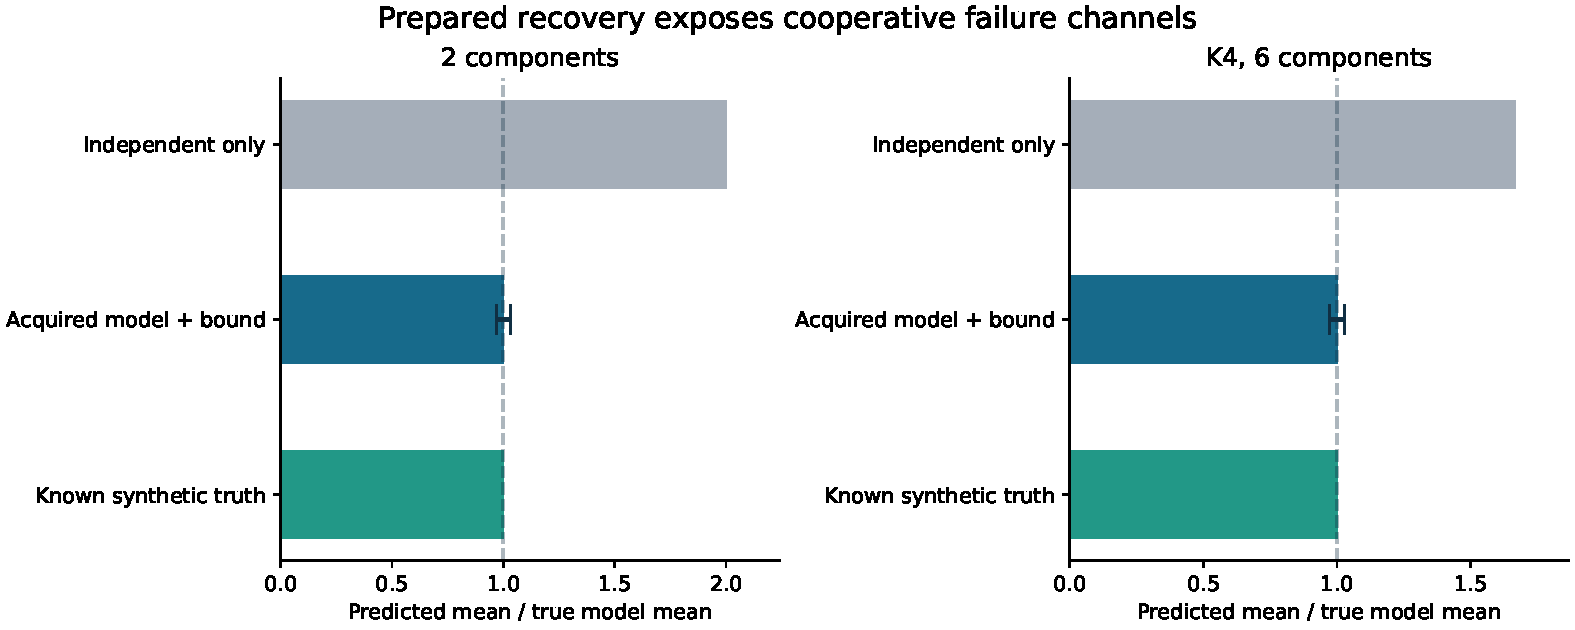
\includegraphics[width=0.93\linewidth]{intervention_results.pdf}
\caption{Synthetic inference compared with the known model means. The independent-only prediction misses the cooperative contribution; the acquired intervals include it. Counts were sampled directly as multinomial totals. The represented trial numbers are not counts of individually executed trajectories or physical laboratory shots.}
\label{fig:results}
\end{figure}

The random seeds are 20261105 and 20261106. The high-precision calculations and eigenvalue diagnostics provide reproducibility checks, not formal interval-arithmetic certification. These intervals omit finite-factory and hardware error because the synthetic experiment uses the exact ideal model. A physical implementation must add those error allocations and use its actual tick duration. In particular, the displayed normalized values are not predictions in seconds for a built device. At leading order in $p$, the $K_4$ independent crossing contribution is $12\gamma p^3$ and the four ports add $8\gamma p^3$, explaining the limiting overestimate $5/3$.

For these particular coefficient ratios, a serial implementation can choose $w_i=1/(m+4r)$ for each refresh and $w_\alpha=4/(m+4r)$ for each additional port. Then $\gamma^{-1}=(m+4r)T$: one displayed time unit is $6T$ for the redundant pair and $22T$ for $K_4$. The padded $T$ must include the finite factory and detector service actually used.

\section{Relation to the strongest applicable existing approaches}
\label{sec:comparison}

\paragraph{Reverse kinetics and multiensemble inference.}
Trendelkamp-Schroer and No\'e's \emph{Efficient Estimation of Rare-Event Kinetics} already infers slow forward kinetics from equilibrium information and downhill simulations, including multistate models and uncertainty \cite{prx2016}. TRAM combines thermodynamic and kinetic information from several ensembles \cite{tram}. Accordingly, neither detailed-balance reversal nor the idea of using prepared high-energy states is a claimed discovery here. The additional guarantee is narrower and more explicit: every transition in a declared finite local reach has a simultaneous absolute interval, the fitted support may omit true channels, and a retained backbone turns those intervals into full fixed-start failure-mean control. The local-table representation and product equilibrium then permit global computation without listing the $2^m$ states. Existing molecular methods apply to much richer interacting landscapes; this note establishes no uniform practical advantage over them.

\paragraph{Accelerated dynamics and mechanism discovery.}
Hyperdynamics and temperature-accelerated dynamics (TAD) accelerate rare events while preserving or reconstructing kinetic information under their respective bias and transition-state assumptions \cite{hyper,tad,tadmath}. TAD can discover mechanisms during elevated-temperature evolution; it is not limited to a pre-enumerated list of actually observed channels. Our distinction is not discovery versus no discovery. It is a different access theorem: unchanged native local collision responses can be prepared and exhaustively covered, with a uniform error budget for mechanisms that remain unobserved. No extrapolation of arbitrary stress-altered rates is made. Conversely, this construction does not supply the continuous potential landscape or transition-state treatment that makes TAD useful in atomistic settings.

\paragraph{Comparison theory, first passage, and network reliability.}
The Dirichlet comparison machinery is classical \cite{comparison}; the local squared-difference and tensorization steps are elementary uses of it. Reactive-flux and spectral rate theory also substantially predate this construction \cite{spectral}. Karger supplies the rare static all-terminal counting algorithm \cite{karger}. The accepted P2 source supplies its conditional self-reduction, short return-avoidance estimator, and independent-network first-failure computation \cite{p2}. We retain those sources as premises. The additions made here are correlated local reversible generators, additive unknown-support acquisition, and a fixed-start perturbation/computation argument without attractiveness when the initial stationary mass is controlled. The sharp independent-component log-rate coefficient from P2 is not asserted for this correlated family.

\paragraph{Other short-trajectory prediction.}
Cheng and Weare prove that temporal-difference methods can have favorable relative asymptotic variance for rare-event prediction from short trajectories \cite{td}. Such results are relevant alternatives to brute-force rare waiting. The present claim is a finite-confidence physical acquisition and succinct-state construction with an explicit network counting component. It does not establish that temporal-difference estimation is inferior on instances where its sampling and representation assumptions are available.

\paragraph{Accumulated Astra interface results.}
The nearby accepted \emph{Port-acquired risk in a hidden thermal family} result controls positive linear Gaussian relaxation mixtures through difference and charge-return protocols \cite{n1607}. It likewise derives what a port can reveal and retains its potentially large guard costs. The present finite local-jump family has a different interface: all local input occupations, unknown discrete support, product equilibrium, and a stochastic backbone. It is not a rebranding of that hidden-relaxation calculation.

\section{Boundaries and the completed consequence}

The interface answers a conditional question about an engineered device. It requires a complete state register and declared local ports, fresh ancillary reset, reciprocal pulses together with the thermal or matched-number conservation condition, a known positive refresh backbone, and protected operations with quantified error. A port's unobserved internal pathways are summed by its measured kernel. Unobserved transitions inside the declared local state table are bounded by confidence intervals. An arbitrary external process is covered by neither statement.

This distinction cannot be removed by more elaborate statistics alone. An additional independent catastrophe of rate $2/M$ appears with probability at most $2T_{\rm obs}/M$ during exposure $T_{\rm obs}$, yet makes the new first-failure mean at most $M/2$. Such a process can break reciprocity, change an unmodeled coordinate, or bypass every instrumented port. A locality, symmetry, reset, or instrument premise is therefore physical information, not evidence manufactured by the inference procedure. Adding a genuinely global unknown port requires paying its global state and preparation costs.

The fixed-start mass condition and mixing contrast are equally substantive. Bare relative form comparison does not, by itself, give a dimension-free relative mean bound from every initial state. A small chance of entering a remote long-lived region can dominate that mean. The explicit $g,\kappa$ bounds prevent that sensitivity from being suppressed in the cost claim. Interacting equilibrium weights, aging, shared repair resources, unobserved history, continuous in-pulse failure, and arbitrary nonthermal faults remain outside the completed theorem.

What is completed is a finite-confidence route from prepared local responses to the mean of a system-level rare first-failure event for this class. It can certify the aggregate effect of channels that were never observed uphill and need not estimate every tiny downhill channel relatively. The numerical examples exhibit a consequential case: the omitted mechanisms change the mean by factors near two and $5/3$, while the acquired full-support intervals retain them. This is a concrete mathematical capability beyond supplying a generator and solving it. Its reach is the derived architecture and error model; hardware realization and broader physical classes are further scientific work.

\paragraph{Reproduction and provenance.}
The accompanying \texttt{rare\_failure\_experiment.py}, \texttt{results.json}, and \texttt{intervention\_results.pdf} contain the synthetic construction, full local counts and intervals, and the plotted output. Running the Python program requires NumPy, SciPy, and Matplotlib. It executes the small-state numerical experiment only. This note is self-contained for the main error and computation proofs while explicitly invoking the corrected Karger subroutine and the governing P2 construction. No historical-priority or civilisation-changing-impact claim is made.

\begin{thebibliography}{99}
\small\raggedright

\bibitem{p2}
Astra Research, \emph{Rare first-failure prediction}, governing P2 package,
fixed revision \texttt{\revhash}, 5 November 2026.
\url{https://github.com/harjassand/astra-research-knowledge/blob/5cfc803599d9f95cfa0a55896fb580e77567e162/research/returns/2026-11-05-p2-first-failure/package/research_note.tex}.

\bibitem{prx2016}
B. Trendelkamp-Schroer and F. No\'e, \emph{Efficient Estimation of Rare-Event Kinetics},
Physical Review X \textbf{6}, 011009 (2016).
\url{https://doi.org/10.1103/PhysRevX.6.011009};
open manuscript \url{https://arxiv.org/abs/1409.6439}.

\bibitem{tram}
H. Wu, F. Paul, C. Wehmeyer, and F. No\'e,
\emph{Multiensemble Markov models of molecular thermodynamics and kinetics},
PNAS \textbf{113}, E3221--E3230 (2016).
\url{https://doi.org/10.1073/pnas.1525092113}.

\bibitem{comparison}
P. Diaconis and L. Saloff-Coste,
\emph{Comparison Theorems for Reversible Markov Chains},
Annals of Applied Probability \textbf{3}, 696--730 (1993).
\url{https://pi.math.cornell.edu/~lsc/papers/comp-rev.pdf}.

\bibitem{karger}
D. R. Karger, \emph{A Randomized Fully Polynomial Time Approximation Scheme for the All-Terminal Network Reliability Problem},
corrected version, SIAM Review \textbf{43}, 499--522 (2001).
\url{https://doi.org/10.1137/S0036144501387141};
\url{https://people.csail.mit.edu/karger/Papers/reliability-sirev.pdf}.

\bibitem{hyper}
A. F. Voter, \emph{Hyperdynamics: Accelerated Molecular Dynamics of Infrequent Events},
Physical Review Letters \textbf{78}, 3908--3911 (1997).
\url{https://doi.org/10.1103/PhysRevLett.78.3908}.

\bibitem{tad}
M. R. S{\o}rensen and A. F. Voter,
\emph{Temperature-accelerated dynamics for simulation of infrequent events},
Journal of Chemical Physics \textbf{112}, 9599--9606 (2000).
\url{https://doi.org/10.1063/1.481576}.

\bibitem{tadmath}
D. Aristoff and T. Leli\`evre, \emph{Mathematical Analysis of Temperature Accelerated Dynamics},
Multiscale Modeling \& Simulation \textbf{12}, 290--317 (2014).
\url{https://doi.org/10.1137/130923063};
\url{https://arxiv.org/abs/1305.6569}.

\bibitem{eto}
M. Lostaglio, A. M. Alhambra, and C. Perry, \emph{Elementary Thermal Operations},
Quantum \textbf{2}, 52 (2018).
\url{https://doi.org/10.22331/q-2018-02-08-52}.

\bibitem{collisions}
J. Ehrich, M. Esposito, F. Barra, and J. M. R. Parrondo,
\emph{Micro-reversibility and thermalization with collisional baths},
Physica A \textbf{552}, 122108 (2020).
\url{https://doi.org/10.1016/j.physa.2019.122108};
\url{https://arxiv.org/abs/1904.07931}.

\bibitem{chaiken}
S. Chaiken, \emph{A Combinatorial Proof of the All Minors Matrix Tree Theorem},
SIAM Journal on Algebraic and Discrete Methods \textbf{3}, 319--329 (1982).
\url{https://doi.org/10.1137/0603033}.

\bibitem{spectral}
J.-H. Prinz, J. D. Chodera, and F. No\'e,
\emph{Spectral Rate Theory for Two-State Kinetics},
Physical Review X \textbf{4}, 011020 (2014).
\url{https://doi.org/10.1103/PhysRevX.4.011020}.

\bibitem{td}
X. Cheng and J. Weare,
\emph{The surprising efficiency of temporal difference learning for rare event prediction},
Advances in Neural Information Processing Systems \textbf{37} (2024).
\url{https://arxiv.org/abs/2405.17638}.

\bibitem{n1607}
Astra Research, \emph{Port-acquired risk in a hidden thermal family},
accepted source N1607, fixed revision \texttt{\revhash}.
\url{https://github.com/harjassand/astra-research-knowledge/blob/5cfc803599d9f95cfa0a55896fb580e77567e162/research/2026-11-01-port-risk-protocol-and-material-reference-renewal/source/p1/FINAL_COMPLETE_14765.txt}.

\end{thebibliography}
\end{document}

